\section{Schichtenmodell}
\subsection{Konsequenzen}
\begin{itemize}
	\item Höhere Ebenen werden einfacher
	\item Änderungen auf höheren Ebenen haben keinen Einfluss auf niedrigere
	\item Änderungen sind unproblematisch, solange die Schnittstelle gleich bleibt
	\item Ebenen sind wiederverwendbar 
	\item Tiefere Ebenen können vor höheren getestet werden
\end{itemize}
$\Rarr$
\begin{itemize}
	\item Reduzierte Komplexität
	\item Verbesserung der Wartbarkeit 
	\item Verbesserung der Portierbarkeit
	\item Verbesserung der Wiederverwendbarkeit
\end{itemize}
\subsection{Schichtenmodell eines DBVS}
\begin{center}
	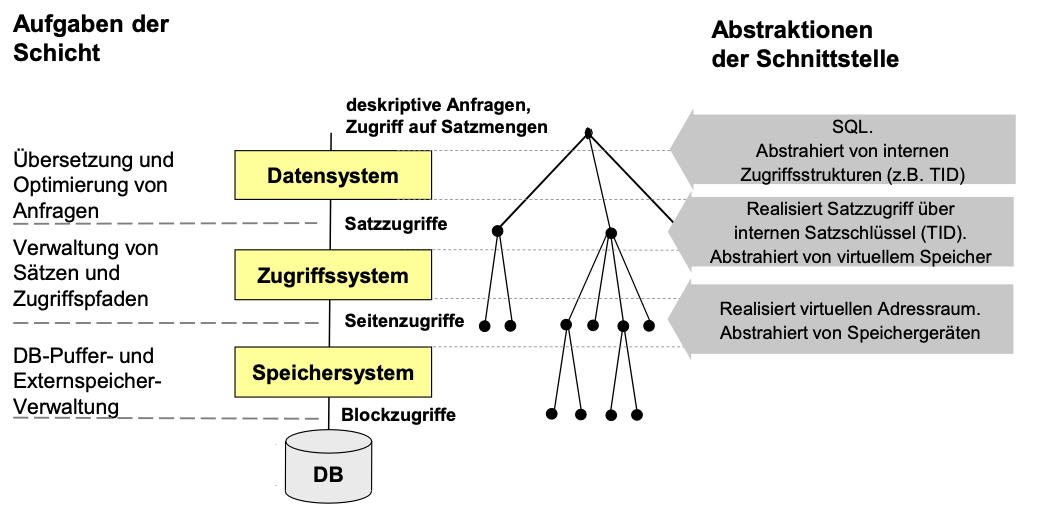
\includegraphics[scale=0.5]{images/Schichtenmodell_Aufgaben.png}
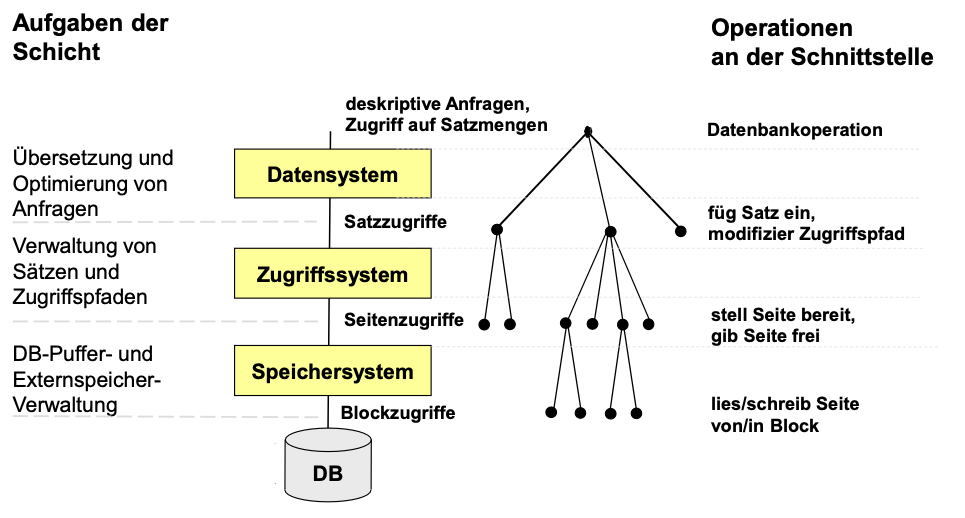
\includegraphics[scale=0.5]{images/Schichtenmodell_Operationen.png}
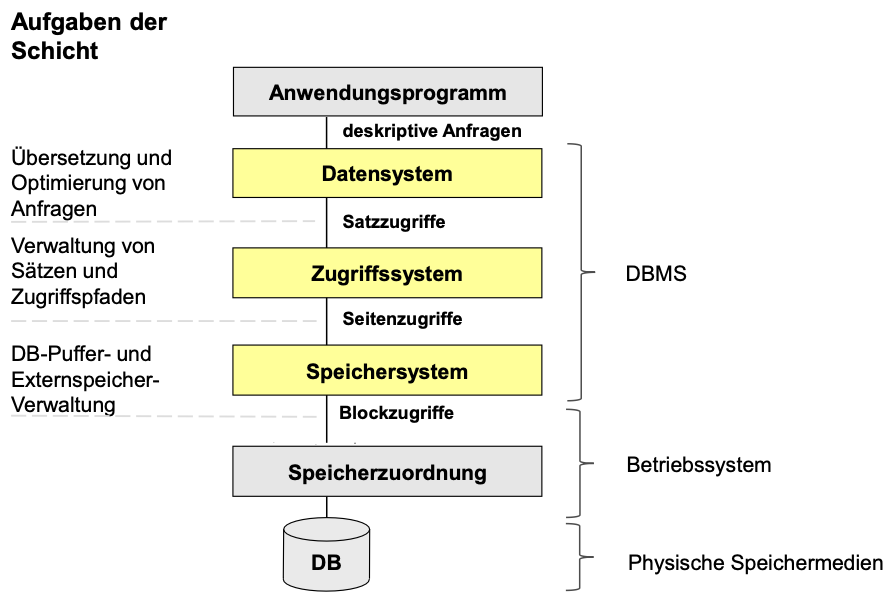
\includegraphics[scale=0.5]{images/Schichtenmodell_Abstraktion.png}
\end{center}
\subsection{Erweitertes Schichtenmodell}
\begin{center}
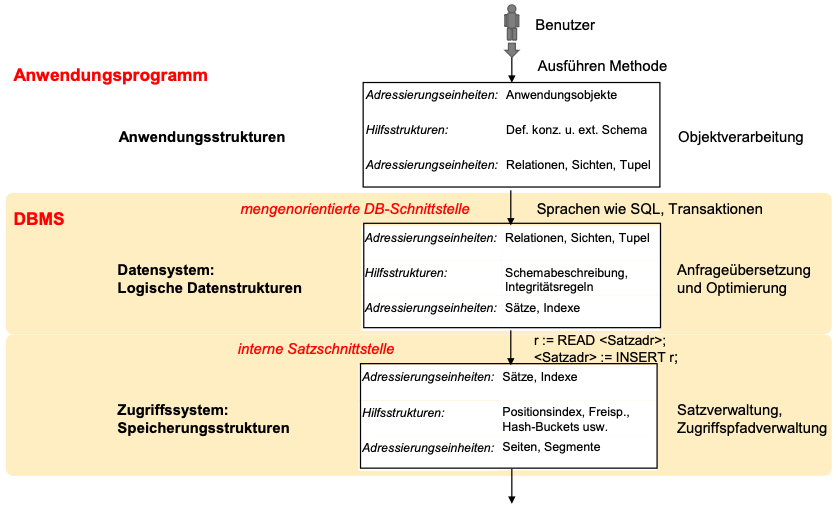
\includegraphics[scale=0.5]{images/Schichtenmodell_erweitert_2.png}
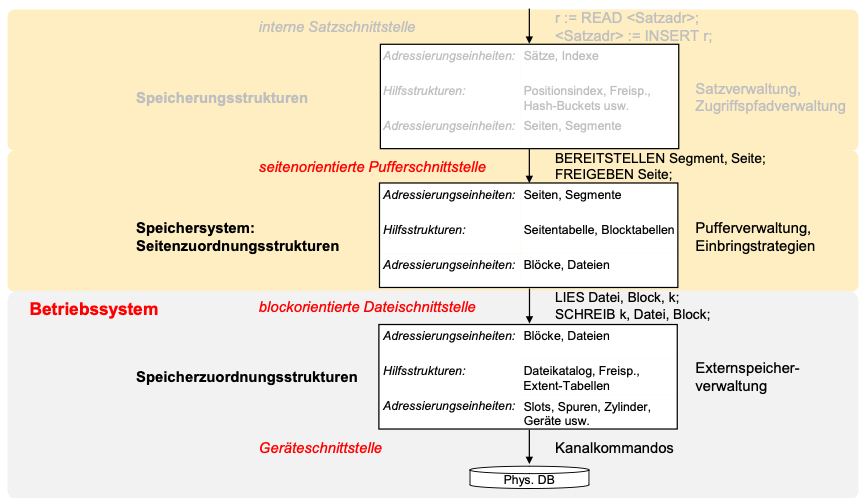
\includegraphics[scale=0.5]{images/Schichtenmodell_erweitert_1.png}
\end{center}
\subsection{Satzadresse}
Eine Satzadresse sollte
\begin{itemize}
	\item eindeutig
	\item unveränderlich
	\item Paar aus Seitennummer und Feldindex
\end{itemize}
sein